% Chapter 1

\chapter{Introducción general} % Main chapter title

\label{Chapter1} % For referencing the chapter elsewhere, use \ref{Chapter1} 
\label{IntroGeneral}
En este capítulo se presentan los principales tipos de pantallas de mensajes variables, las características de las pantallas \textit{full color} y por último se explica la motivación, el alcance y objetivos de este trabajo.
%----------------------------------------------------------------------------------------

% Define some commands to keep the formatting separated from the content 
\newcommand{\keyword}[1]{\textbf{#1}}
\newcommand{\tabhead}[1]{\textbf{#1}}
\newcommand{\code}[1]{\texttt{#1}}
\newcommand{\file}[1]{\texttt{\bfseries#1}}
\newcommand{\option}[1]{\texttt{\itshape#1}}
\newcommand{\grados}{$^{\circ}$}

%----------------------------------------------------------------------------------------

%\section{Introducción}

%----------------------------------------------------------------------------------------
\section{Pantallas de mensaje variable}

Los paneles de mensajes variables son señales de tránsito diseñadas para alertar o informar a los conductores. La pantalla de mensajes variables puede mostrar pictogramas o mensajes escritos. Las imágenes en pantalla pueden ser estáticas, parpadeantes o realizar efectos \cite{WIKIVMS}.


\subsection{Pantallas fijas}

Las pantallas fijas de mensajes variables generalmente se montan en estructuras aéreas que abarcan en voladizo una parte de la carretera, o fuera de la carretera. Se utilizan para influir en los conductores con propósitos de control de tránsito. Sus mensajes pueden cambiarse manual, mecánica o electromecánicamente para proporcionar a los automovilistas información sobre congestión del tráfico, accidentes de tráfico, operaciones de mantenimiento, condiciones climáticas adversas, condiciones de la carretera, eventos organizados u otras características de la vía. Un beneficio de las pantallas fijas de mensaje variable es que pueden desplegar mensajes más detallados y permitir un adecuado tiempo de exposición  para que los automovilistas comprendan los mensajes antes de llegar a un punto de decisión. En la figura \ref{fig:vmsp} se muestra una pantalla fija de mensajes variables \citep{VMSTYPES}.



\subsection{Pantallas móviles}

Las pantallas móviles de mensajes variables suelen estar montadas en un remolque con paneles solares, son de fácil movimiento y pueden ser colocadas cerca de puntos de decisión donde el conductor puede realizar una acción como por ejemplo tomar un camino alterno o disminuir la velocidad. Sus mensajes se pueden cambiar de forma manual, mecánica o por medios electromecánicos. Un beneficio de los paneles de mensajes variables móviles es la posibilidad de ubicación en puntos estratégicos. En la figura \ref{fig:vmsm} se muestra una pantalla móvil de mensajes variables \citep{VMSTYPES}.

\begin{figure}[htpb]
	\centering
	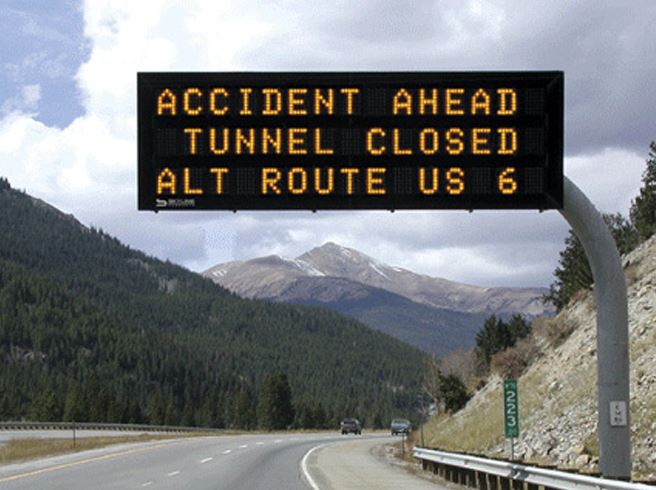
\includegraphics[width=.9 \textwidth]{../Figures/vmspermanente.jpg} 
	\caption{Pantalla fija \protect\footnotemark.}
	\label{fig:vmsp}
\end{figure}

\footnotetext{Imagen tomada de \url{https://www.skylineproducts.com/wp-content/uploads/2016/07/Walk-In.jpg}}

\begin{figure}[htpb]
	\centering
	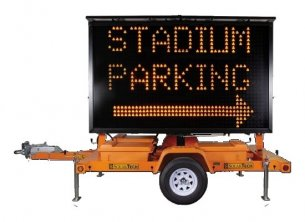
\includegraphics[width=.7\textwidth]{../Figures/vmsmovil.jpg} 
	\caption{Pantalla móvil \protect\footnotemark.}
	\label{fig:vmsm}
\end{figure}
\footnotetext{Imagen tomada de \url{https://www.enterpriseflasher.com/assets/images/solartech-1364402479.jpg}}

\pagebreak
\subsection{Pantallas montadas en camión}

Las pantallas de mensajes variables montadas en camión son generalmente unidades pequeñas ubicadas en o cerca de la parte trasera de un camión. Los paneles montados en camión generalmente tienen espacio reducido para mensajes. Las limitaciones de sus mensajes suelen resultar en el uso de gráficos como flechas para facilitar la comprensión del conductor \citep{VMSTYPES}. En la figura \ref{fig:vmsc} se muestra una pantalla montada en un camión.

\begin{figure}[htpb]
	\centering
	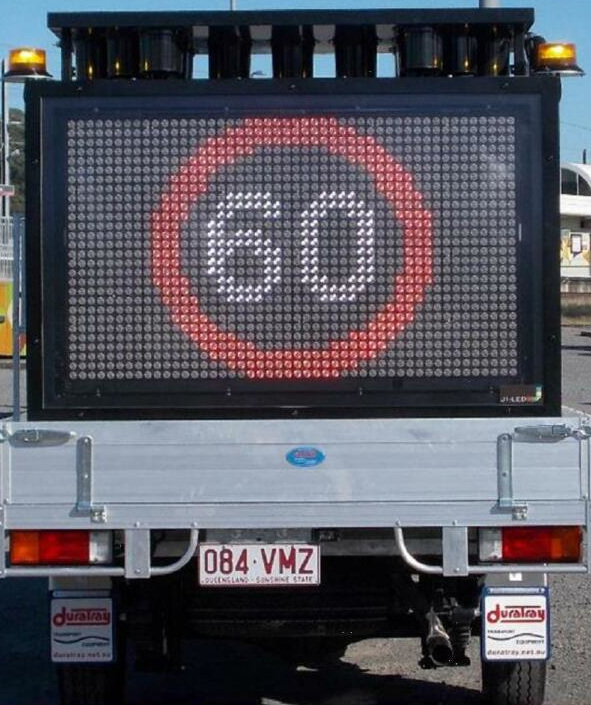
\includegraphics[scale=1]{../Figures/vmstruck.png} 
	\caption{Pantalla montada en camión \protect\footnotemark.}
	\label{fig:vmsc}
\end{figure}
\footnotetext{Imagen tomada de  \url{https://www.mobilesystems.co.nz/vdb/image/i2123}}


\section{Pantalla full color}
La pantalla de \textit{full color} es un dispositivo electrónico compuesto por arreglos matriciales de LEDs. Dichos LEDs forman píxeles. Con los píxeles se puede formar textos, imágenes y hasta vídeo. Las pantallas LED se fabrican de una forma modular con el propósito de facilitar la instalación, transporte y mantenimiento. A continuación se enumeran algunas de las características de una pantalla \textit{full color} \citep{WIKIPANTALLAFULLCOLOR}. En la figura \ref{fig:grafrgb} se muestra una representación gráfica del modelo RGB.


\subsection{Full color}
\textit{Full color} es un término que significa que los colores primarios (rojo, verde y azul ) se mezclan para producir millones de tonos individuales. Se utiliza frecuentemente el modelo RGB en donde cada color es la suma de los primarios rojo, verde y azul. Mediante la mezcla de estos tres con diferente intensidad se representan distintos colores.



\subsection{Resolución de pantalla}
La resolución de una pantalla se define como la cantidad de píxeles que esta posee. Se expresa como el producto de la cantidad de filas por el número de columnas \citep{WIKIRESOL}. Mientras mayor sea la resolución mayor cantidad de detalles se podrán apreciar en la imagen como se muestra en la figura \ref{fig:grafresolucion}.

\begin{figure}[htpb]
	\centering
	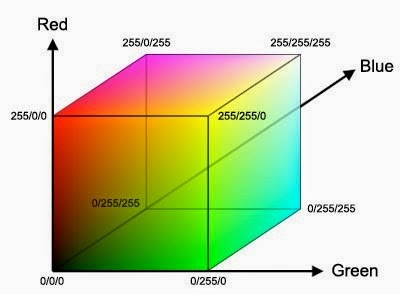
\includegraphics[scale=0.6]{Figures/modelorgb.jpg} 
	\caption{Modelo RGB\protect\footnotemark.}
	\label{fig:grafrgb}
\end{figure}
\footnotetext{Imagen tomada de \url{http://3.bp.blogspot.com/-NiYCndNGwHk/VCT\_ ywjC8FI/AAAAAAAAApk/0WDDtMziu6I/s1600/RGB1.jpg}}

\begin{figure}[htpb]
	\centering
	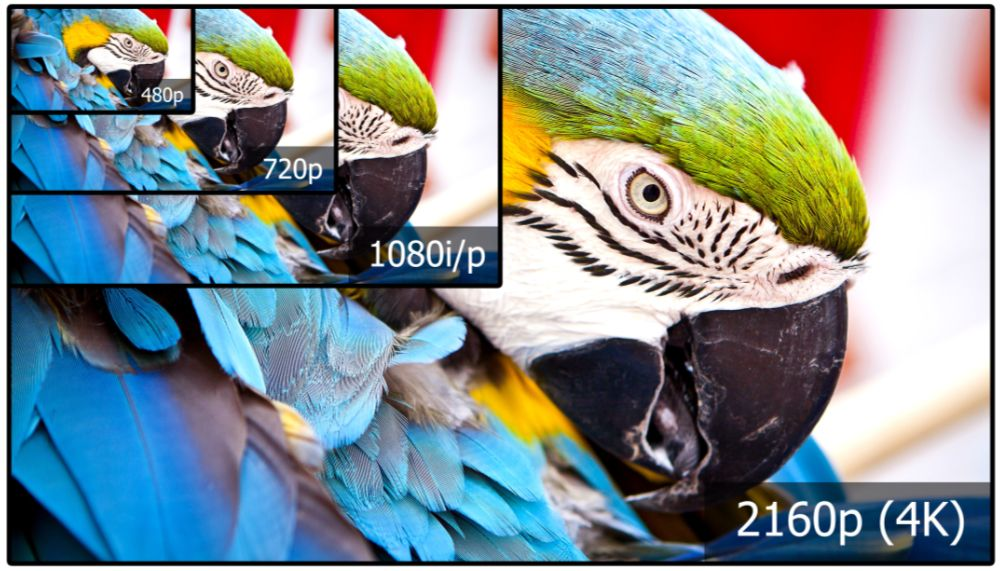
\includegraphics[scale=0.3]{Figures/resolucion.jpg} 
	\caption{Representación gráfica de resolución\protect\footnotemark.}
	\label{fig:grafresolucion}
\end{figure}
\footnotetext{Imagen tomada de \url{https://www.4kmonitor.net/wp-content/uploads/2020/03/4K-Monitor-Vor-und-Nachteile.jpg}}

\subsection{Píxel pitch}
Se define \textit{píxel pitch} a la distancia física que separa a los LEDs que conforman la pantalla. Esta distancia es medida en milímetros. La resolución de la pantalla tiene relación directa con el \textit{pitch}. Mientras más pequeño sea el \textit{pitch} mayor será la resolución para un mismo tamaño de pantalla \citep{IMAGENDEF2}. La figura \ref{fig:pixelpitch} muestra paneles LED en los que se resalta el \textit{pitch}.

Se suele abreviar esta medida con un "P-" seguida de la medida en milímetros. Por ejemplo ,la pantalla de esta memoria es una pantalla P-20.



\subsection{Tamaño de pantallas gigantes}
No existe ningún estándar para definir el tamaño de las pantallas gigantes. Las pantallas LED  se pueden construir uniendo módulos hasta alcanzar el tamaño deseado. La selección del \textit{pitch} de las pantalla gigantes para exteriores depende de la distancia del espectador como se puede observar en la figura \ref{fig:pitchview}.

\begin{figure}[htpb]
	\centering
	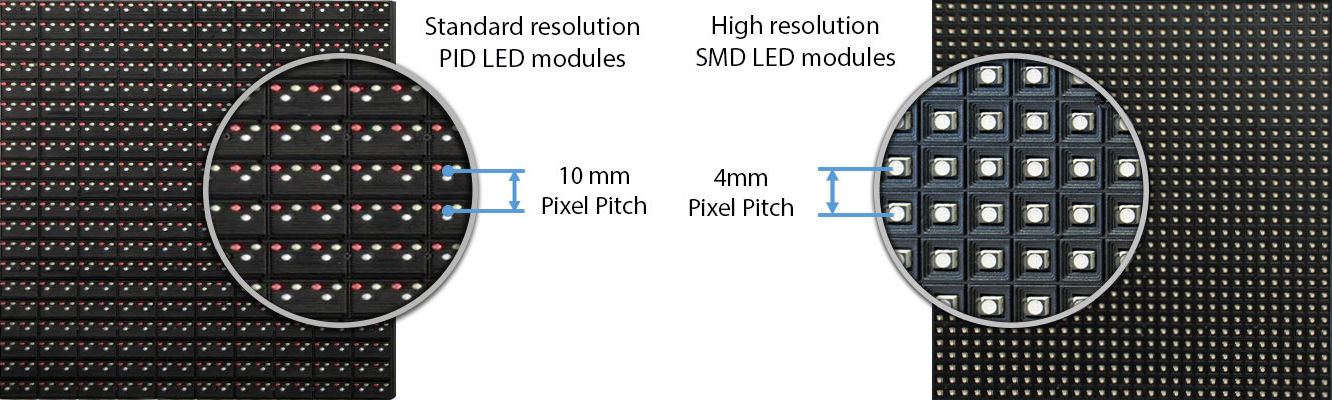
\includegraphics[scale=0.3]{Figures/pitch.jpg} 
	\caption{Representación gráfica de \textit{pitch}\protect\footnotemark.}
	\label{fig:pixelpitch}
\end{figure}
\footnotetext{Imagen tomada de \url{https://www.finepixelled.com/theme/basic-knowledge/pixel-pitch-resolution.jpg}}

\begin{figure}[htpb]
	\centering
	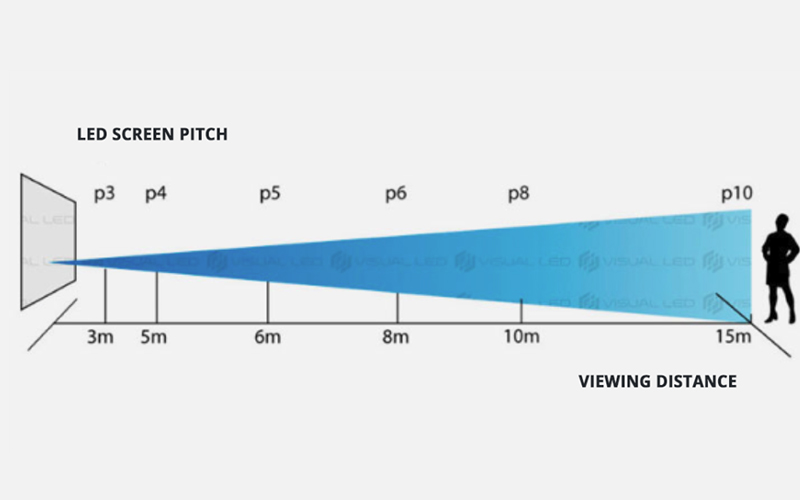
\includegraphics[scale=0.6]{Figures/visionpitch.jpg} 
	\caption{Selección de \textit{pitch} de acuerdo a la distancia del espectador \protect\footnotemark.}
	\label{fig:pitchview}
\end{figure}
\footnotetext{Imagen tomada de \url{https://www.doitvision.com/wp-content/uploads/2020/07/led-display-visual-distance.jpg}}

\pagebreak




\section{Paneles informativos comerciales}
Existe una gran cantidad de fabricantes de pantallas LED P-20 para exteriores. El país líder en producción de pantallas LED para exteriores es China. En la tabla \ref{tab:comercial} se muestra una comparación de las características de algunas pantallas comerciales. De esta comparación se puede observar que las pantallas comparten características muy similares a excepción del consumo de energía que está relacionado con el tipo de LED que se usa para construir la pantalla. 

\begin{table}[h]
\centering
\caption[Comparación entre pantallas P-20]{Comparación de características de pantallas P-20 comerciales.}
\begin{tabular}{l c c c}
\toprule
\textbf{Característica} & \textbf{S. Chuangkaiguang Co \citep{TABLAREF1}} & \textbf{Leeman \citep{TABLAREF2}} & \textbf{Samsung \citep{TABLAREF3}} \\
\midrule 

Ángulo de visión        & H120, V60 & H120, V60 & H140, V59 \\
Constitución de píxel   & RGB & RGB & RGB \\
Tasa de refresco        & mayor a 60 Hz & 60 Hz & 60 Hz \\
Consumo promedio        & \SI{200}{\watt\per\meter\squared} & \SI{200}{\watt\per\meter\squared} & \SI{169}{\watt\per\meter\squared} \\
Grado de protección     & IP65 & IP65 & IP65 \\

\bottomrule
\hline
\end{tabular}
\label{tab:comercial}
\end{table}





\section{Motivación}
Existieron muchos motivos que llevaron a la creación de una pantalla \textit{full color gigante}. El motivo principal fue la necesidad de desarrollar y construir productos de alto valor agregado de manera local. Dentro de Ecuador no existe ninguna empresa que construya pantallas gigantes. Existen muchas empresas dedicadas a comercializar pantallas importadas. 

Otro de los motivos es que en Ecuador los impuestos de importación a productos terminados es muy alto. Construir la pantalla en el país es una opción viable gracias a estos impuestos. El tercer motivo es la representación local del producto, ya que la empresa se encuentra dentro del país y puede garantizar el servicio técnico durante el tiempo del contrato. Finalmente desarrollar una pantalla LED \textit{full color} fue un reto personal que forma parte de mi desarrollo profesional. 



\section{Propósito del trabajo}
El propósito de este trabajo fue desarrollar una pantalla gigante \textit{full color} LED. Se espera que el desarrollo de este nuevo producto diversifique el portafolio de productos viales que ya posee la empresa.

\pagebreak

\section{Alcance del trabajo}
El presente trabajo incluye:

\begin{itemize}
\item Diseño y construcción de una pantalla LED de 384 por 96 píxeles.
\item Manuales de ensamblaje eléctrico de la pantalla.
\item Desarrollo de firmware de la pantalla.
%\footnotetext{Referencia de placa  https://www.terasic.com.tw/cgi-bin/page/archive.pl?Language=English\&No=836}


\end{itemize}

El presente trabajo no incluye:

 \begin{itemize}
\item La interfaz gráfica para el cargado remoto de la imágenes.
\item La aplicación para cargar imágenes en forma local.
\item Diseño de ventilación 
\item Diseño de mecánica de armado.

\end{itemize}




